% Relaxing S_hc for the Fig. 1 transmon-resonator example: the compact phase varphi_1 and the
% harmonic resonator phase varphi_2 live on a cylinder. (a) The physical cylinder; (b) the strip
% cut open in sheared coordinates varphi_1 = varphi_u, varphi_2 = varphi_v + alpha varphi_u, whose edges are sewn
% with an offset; (c) the charges, where the integer transmon charge n_u - alpha n_v puts the
% allowed states on tilted lines and n_v stays continuous.
% Adapted from Notes/figs/compact_shear_cylinder.tex (panels a and c).
% Compile standalone with the draw-circuit driver; \input into main.tex via the standalone package.
\documentclass[border=9pt]{standalone}
\usepackage{amsmath,amssymb}
\usepackage{tikz}
\definecolor{figBlue}{RGB}{0,114,178}
\definecolor{figOrange}{RGB}{213,94,0}
\begin{document}
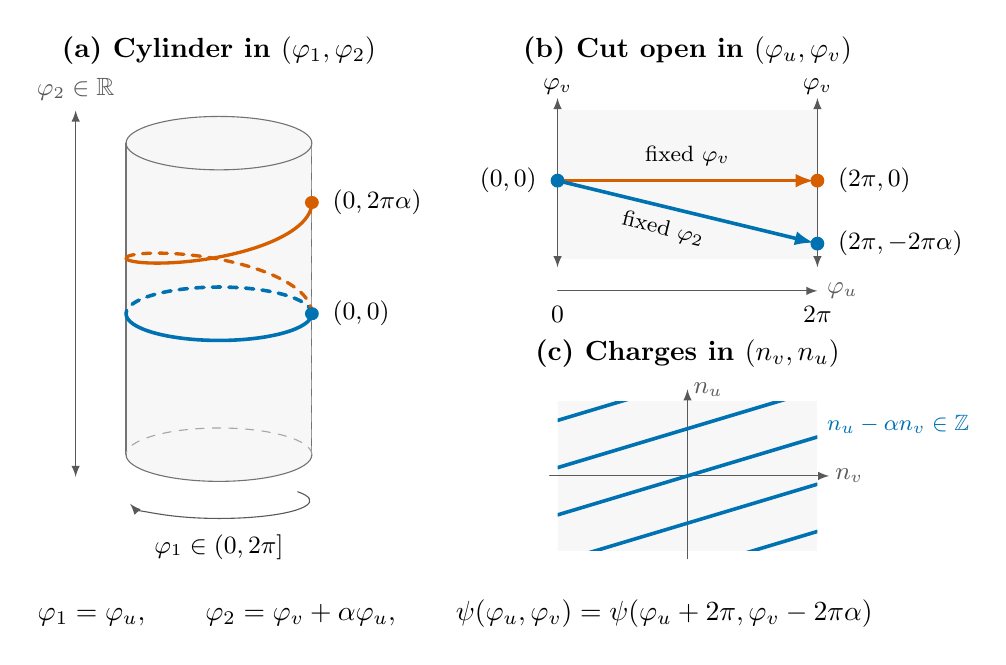
\begin{tikzpicture}[font=\small,>=latex,line cap=round,line join=round]
\node[font=\bfseries] at (1.7,6.2) {(a) Cylinder in $(\varphi_1,\varphi_2)$};
\begin{scope}[yshift=0.128cm,yscale=0.942]
\fill[black!3] (0.52,1) -- (0.52,5.2) arc[start angle=180,end angle=0,x radius=1.18,y radius=0.36] -- (2.88,1) arc[start angle=0,end angle=-180,x radius=1.18,y radius=0.36];
\draw[black!55] (0.52,1) -- (0.52,5.2) (2.88,1) -- (2.88,5.2);
\draw[black!55] (1.7,5.2) ellipse[x radius=1.18,y radius=0.36];
\draw[black!35,dashed] (2.88,1) arc[start angle=0,end angle=180,x radius=1.18,y radius=0.36];
\draw[black!55] (2.88,1) arc[start angle=0,end angle=-180,x radius=1.18,y radius=0.36];
\draw[black!40,dashed] (2.88,1) -- (2.88,5.2);
\draw[figBlue,line width=1.3pt,dashed] (2.88,2.9) arc[start angle=0,end angle=180,x radius=1.18,y radius=0.36];
\draw[figBlue,line width=1.3pt] (2.88,2.9) arc[start angle=0,end angle=-180,x radius=1.18,y radius=0.36];
\draw[figOrange,line width=1.2pt,dashed] plot[smooth] coordinates {(2.8800,2.9000) (2.8793,2.9209) (2.8771,2.9418) (2.8735,2.9626) (2.8685,2.9834) (2.8621,3.0042) (2.8542,3.0248) (2.8449,3.0454) (2.8343,3.0659) (2.8222,3.0862) (2.8088,3.1065) (2.7941,3.1265) (2.7780,3.1464) (2.7606,3.1661) (2.7419,3.1857) (2.7219,3.2050) (2.7007,3.2241) (2.6783,3.2430) (2.6546,3.2616) (2.6299,3.2800) (2.6039,3.2981) (2.5769,3.3159) (2.5488,3.3334) (2.5197,3.3506) (2.4896,3.3675) (2.4585,3.3841) (2.4265,3.4004) (2.3936,3.4162) (2.3598,3.4318) (2.3253,3.4470) (2.2900,3.4618) (2.2540,3.4762) (2.2173,3.4902) (2.1799,3.5039) (2.1420,3.5171) (2.1036,3.5300) (2.0646,3.5424) (2.0253,3.5544) (1.9855,3.5660) (1.9453,3.5771) (1.9049,3.5879) (1.8642,3.5982) (1.8233,3.6080) (1.7823,3.6175) (1.7412,3.6264) (1.7000,3.6350) (1.6588,3.6431) (1.6177,3.6508) (1.5767,3.6580) (1.5358,3.6648) (1.4951,3.6712) (1.4547,3.6771) (1.4145,3.6826) (1.3747,3.6877) (1.3354,3.6924) (1.2964,3.6966) (1.2580,3.7005) (1.2201,3.7039) (1.1827,3.7069) (1.1460,3.7095) (1.1100,3.7118) (1.0747,3.7136) (1.0402,3.7151) (1.0064,3.7162) (0.9735,3.7170) (0.9415,3.7174) (0.9104,3.7175) (0.8803,3.7173) (0.8512,3.7167) (0.8231,3.7159) (0.7961,3.7147) (0.7701,3.7133) (0.7454,3.7116) (0.7217,3.7096) (0.6993,3.7074) (0.6781,3.7050) (0.6581,3.7023) (0.6394,3.6995) (0.6220,3.6964) (0.6059,3.6932) (0.5912,3.6898) (0.5778,3.6862) (0.5657,3.6826) (0.5551,3.6788) (0.5458,3.6748) (0.5379,3.6708) (0.5315,3.6668) (0.5265,3.6626) (0.5229,3.6584) (0.5207,3.6542) (0.5200,3.6500)};
\draw[figOrange,line width=1.2pt] plot[smooth] coordinates {(0.5200,3.6500) (0.5207,3.6458) (0.5229,3.6416) (0.5265,3.6374) (0.5315,3.6332) (0.5379,3.6292) (0.5458,3.6252) (0.5551,3.6212) (0.5657,3.6174) (0.5778,3.6138) (0.5912,3.6102) (0.6059,3.6068) (0.6220,3.6036) (0.6394,3.6005) (0.6581,3.5977) (0.6781,3.5950) (0.6993,3.5926) (0.7217,3.5904) (0.7454,3.5884) (0.7701,3.5867) (0.7961,3.5853) (0.8231,3.5841) (0.8512,3.5833) (0.8803,3.5827) (0.9104,3.5825) (0.9415,3.5826) (0.9735,3.5830) (1.0064,3.5838) (1.0402,3.5849) (1.0747,3.5864) (1.1100,3.5882) (1.1460,3.5905) (1.1827,3.5931) (1.2201,3.5961) (1.2580,3.5995) (1.2964,3.6034) (1.3354,3.6076) (1.3747,3.6123) (1.4145,3.6174) (1.4547,3.6229) (1.4951,3.6288) (1.5358,3.6352) (1.5767,3.6420) (1.6177,3.6492) (1.6588,3.6569) (1.7000,3.6650) (1.7412,3.6736) (1.7823,3.6825) (1.8233,3.6920) (1.8642,3.7018) (1.9049,3.7121) (1.9453,3.7229) (1.9855,3.7340) (2.0253,3.7456) (2.0646,3.7576) (2.1036,3.7700) (2.1420,3.7829) (2.1799,3.7961) (2.2173,3.8098) (2.2540,3.8238) (2.2900,3.8382) (2.3253,3.8530) (2.3598,3.8682) (2.3936,3.8838) (2.4265,3.8996) (2.4585,3.9159) (2.4896,3.9325) (2.5197,3.9494) (2.5488,3.9666) (2.5769,3.9841) (2.6039,4.0019) (2.6299,4.0200) (2.6546,4.0384) (2.6783,4.0570) (2.7007,4.0759) (2.7219,4.0950) (2.7419,4.1143) (2.7606,4.1339) (2.7780,4.1536) (2.7941,4.1735) (2.8088,4.1935) (2.8222,4.2138) (2.8343,4.2341) (2.8449,4.2546) (2.8542,4.2752) (2.8621,4.2958) (2.8685,4.3166) (2.8735,4.3374) (2.8771,4.3582) (2.8793,4.3791) (2.8800,4.4000)};
\fill[figBlue] (2.88,2.9) circle(2.5pt);
\node[right=4pt] at (2.88,2.9) {$(0,0)$};
\fill[figOrange] (2.88,4.4) circle(2.5pt);
\node[right=4pt] at (2.88,4.4) {$(0,2\pi\alpha)$};
\draw[<->,black!65] (-0.12,0.7) -- (-0.12,5.640) node[above] {$\varphi_2\in\mathbb R$};
\draw[->,black!65] (2.7,0.5) arc[start angle=30,end angle=-170,x radius=1.15,y radius=0.24];
\node at (1.7,-0.242) {$\varphi_1\in(0,2\pi]$};
\end{scope}
\begin{scope}[xshift=6.0cm]
% (b) strip at half height
\node[font=\bfseries] at (1.65,6.2) {(b) Cut open in $(\varphi_u,\varphi_v)$};
\fill[black!3] (0,3.55) rectangle (3.3,5.45);
\draw[<->,black!65] (0,3.45) -- (0,5.6);
\draw[<->,black!65] (3.3,3.45) -- (3.3,5.6);
\node[above,inner sep=1pt] at (0,5.6) {$\varphi_v$};
\node[above,inner sep=1pt] at (3.3,5.6) {$\varphi_v$};
\draw[->,figOrange,line width=1.2pt] (0,4.55) -- (3.25,4.55);
\node[above=2pt,font=\footnotesize] at (1.65,4.55) {fixed $\varphi_v$};
\draw[->,figBlue,line width=1.3pt] (0,4.55) -- (3.25,3.762);
\node[below=1pt,rotate=-13.6,font=\footnotesize] at (1.4,4.21) {fixed $\varphi_2$};
\fill[figBlue] (0,4.55) circle(2.5pt) (3.3,3.75) circle(2.5pt);
\fill[figOrange] (3.3,4.55) circle(2.5pt);
\node[left=4pt] at (0,4.55) {$(0,0)$};
\node[right=4pt] at (3.3,3.75) {$(2\pi,-2\pi\alpha)$};
\node[right=4pt] at (3.3,4.55) {$(2\pi,0)$};
\draw[->,black!65] (0,3.15) -- (3.3,3.15) node[right] {$\varphi_u$};
\node[below=2pt] at (0,3.15) {$0$};
\node[below=2pt] at (3.3,3.15) {$2\pi$};
% (c) charge plane: allowed states n_1 = n_u - alpha n_v in Z (blue); n_v stays continuous
\node[font=\bfseries] at (1.65,2.35) {(c) Charges in $(n_v,n_u)$};
\fill[black!3] (0,-0.15) rectangle (3.3,1.75);
\draw[->,black!65] (-0.1,0.8) -- (3.45,0.8) node[right,inner sep=2pt] {$n_v$};
\draw[->,black!65] (1.65,-0.25) -- (1.65,1.9) node[right,inner sep=2pt] {$n_u$};
\begin{scope}
\clip (0,-0.15) rectangle (3.3,1.75);
\foreach \m in {-3,...,3} {
  \draw[figBlue,line width=1.3pt] (0,0.8+0.6*\m-0.495) -- (3.3,0.8+0.6*\m+0.495);
}
\end{scope}
\node[right,figBlue,font=\footnotesize] at (3.3,1.45) {$n_u-\alpha n_v\in\mathbb Z$};
\end{scope}
\node[align=center,font=\normalsize] at (4.7,-0.95) {$\varphi_1=\varphi_u,\qquad \varphi_2=\varphi_v+\alpha \varphi_u,\qquad
\psi(\varphi_u,\varphi_v)=\psi(\varphi_u+2\pi,\varphi_v-2\pi\alpha)$};
\end{tikzpicture}
\end{document}
